\chapter{Design of Experiments}
\chaptermark{DOE}

This chapter is devoted to the matter of designing experiments, and follows the lines of \cite{cox_theory_2000}.
A control chart may be seen as an on-line experiment alerting us when the milk goes sour, but it will not tell us why. 
When designing a product (remember DFSS \ref{sec:dfss}), or once a control chart has signalled an alert, we will want to know what has influences our production, and how to remove variability.
In our SPC terminology, we will want to know what are the \emph{causal} \emph{effects} of our \emph{controllable inputs} (or \emph{factors}), on our \emph{CTQ} (or \emph{response}). 
The theory of discovering these effects is the theory of \emph{design of experiments} (DOE).
Its goal is to \emph{screen} factors with no effect, to estimate effect sizes, and find optimal factor-level combinations, and remove assignable variability; all these as efficiently as possibly.



Roughly speaking, the challenges in designing good experiment are:
\begin{enumerate}
\item Efficiency: extract the most information per sample. 
\item Signal to noise: remove variability that might mask factor effects.
\item Bias: avoid uncontrolled factor-effects from being ``absorbed'' into controlled factor effects.
\end{enumerate}





Before we dig in, several matters should be emphasized:
\begin{description}
\item [Randomization] Randomization is fundamental to our purpose. This because the idea of an \emph{effect} implies causality. Any inference we make, is causal, which is the inference we need for controlling a process.
It is the mechanism of randomization, that allows us to conclude that inferred correlations are causal, and not merely statistical.
For a treatment of causal inference in \emph{observational data}, i.e., without randomization, see \cite{rosenbaum_observational_2002}.

\item [Pre-experiment] In this text we take it for granted that the purpose of the experiment is well known, and the candidate factors defined. We are fully aware, as should be the reader, that in application this is a non-trivial luxury. Indeed, a lot of planning, and domain-knowledge go into the selection of factors, their candidate levels, etc.

\item [Power Analysis] Part of the pre-experiment may include a power analysis. The pre-experiment power analysis will typically be very approximate, and rely on many assumptions. It is still important, as it gives an idea of the feasibility of an experiment, and avoids wasting resources.

\item [No Textbook Solution] We will present many design ideas and principles, yet it should be emphasized that real life problems rarely obey text-books. You should thus feel free, and even obliged, to think about your particular problem and adapt the experiment as you best see fit. 

\item[Data Analysis]
In this text, we only discuss the \textbf{design} of the experiment, and not the \textbf{analysis} of the data.
This is a non-standard choice as DOE is typically presented alongside the \emph{analysis of variance} (ANOVA) framework.\marginnote{ANOVA}
We decouple the two since: 
\cite{cox_theory_2000} do so, 
these are two different thing, and finally, because the ANOVA framework may be easily replaced by the framework of \emph{linear models}, \emph{mixed models}, \emph{variance components}, and possibly others. 
There is a vast literature focusing on the analysis method. \marginnote{Linear Models, \\ Mixed Models, Variance Components}
If asked, this author may recommend \cite{hocking_analysis_1985}, which presents both the ANOVA terminology, and the linear models terminology.
That book, however, may be hard to come by, so feel free to ask me for other references if required.

\end{description}








\section{Terminology}
The following list is compiled from \cite{mason_statistical_2003}. Many, if not most of the following terms, originate in R.A. Fisher's seminal book ``The Design of Experiments'' \citep{fisher_design_1960}. As usual, when old ideas get new names, we try to emphasize this in the text.



\begin{description}

\item [Experimental Unit]  Entity on which a measurement or an observation is made;
sometimes refers to the actual measurement or observation.
\item [Homogenous Experimental Unit] Units that are as uniform as possible on all characteristics that could affect the response.

\item [Factors]  A controllable experimental variable that is thought to influence the response. In the language of SPC: \emph{a controllable input}.

\item [Level] Specific value of a factor.

\item[Treatment] The particular factor-level combination applied to an experimental unit. \Aka \emph{manipulation}.

\item [Factor Encodings] The numerical encoding of factor levels.
Of minor importance for designing. Of major importance for analysis.
Two level factor encodings include:
\begin{enumerate}
\item Effect coding: where levels are encoded with $-1,1$ returning orthogonal design matrices for balanced designs.
\item Dummy coding: where levels are encoded with $0,1$ returning easily interpretable coefficients.
\end{enumerate}

\item [Experimental Region] All possible factor–level combinations for which experimentation is possible. \Aka \emph{factor space}, and \emph{design region}.

\item [Design Matrix] A matrix description of an experiment that is useful for constructing and analyzing experiments.

\item [Response] The CTQ.

\item [Main Effect] Change in the expected response between two factor–levels.  We emphasize that effects, unlike simple population parameters, imply a causal relationship.

\item [Interaction] Existence of joint factor effects in which the effect of each factor depends on the levels of the other factors.

\item [Replication] Repetition of an entire experiment or a portion of an experiment under two or more sets of conditions.

\item [Covariate]  An uncontrollable variable that influences the response but is
unaffected by any other experimental factors.

\item [Design]  Complete specification of experimental test runs, including blocking, randomization, repeat tests, replication, and the assignment of factor–level combinations to experimental units.

\item [Blocking]  Blocking, or \emph{grouping}, is an experimental design technique that removes excess variation by grouping experimental units or test runs so that those units or test runs within a block are more homogeneous than those in different blocks. Blocking attributes are also known as \emph{non specific factors}.\marginnote{Non Specific Factors}

\item [Confounding] When the design is such that several effects cannot be told apart. \Aka \emph{aliasing}.

\item [Repeat Tests] Two or more observations that have the same levels for all the factors.

\item [Balance] Some symmetry in the combinatorial design of the experiment. In its simplest interpretation, a design where an equal number of units is assigned to each treatment.

\item [Orthogonality]  Special simplifications of analysis and achievement of efficiency consequent on such \emph{balance}.
\end{description}








\section{Dealing with Variability}
\label{sec:variance_components}

The idea that random samples come with variability, or noise, should not be new to the reader (but see Extra~\ref{extra:pac_learning} below.)
In this section, we will try to decompose variability into it sources, and learn several techniques to reduce the noise sources. 
Starting with a motivating example.



\begin{example}[Movie Ratings]
\label{eg:variance_components}
Consider the problem of ranking movies along their rating.
For this purpose, individuals are asked to rate each movie they have seen.
A movie's rating is thus influenced by several factors:
the movie's quality, 
the viewer's general tastes, 
the viewer's particular tastes to that type of movie,
the viewer's mood at the time of watching,
other factors.
How can we accurately rate a movie, in the presence of these variability sources?
The movie's quality is a controllable input, thus a factor.
The viewer's strictness is not controllable, but observable, thus may be introduced as a covariate.
The viewer's affinity to that type of movie is an interaction, since both movie type and viewer, are observable.
The viewer's mood is unobservable, but we certainly acknowledge its existence. 
Any other variance source, will be captured by the error term of the model. 
\end{example}

Example~\ref{eg:variance_components} teaches us that by an informed experimental design and analysis, we may reduce noise.
Either by moving it to the signal (with covariates), or by trying to reduce it.
These are the ideas discussed in this section.


\begin{extra}[PAC learning]
\label{extra:pac_learning}
It may be shocking for a statistician, but not all data is assumed noisy.
Try reading about \emph{PAC learning} in the machine learning literature for a counter example.
\end{extra}




\subsection{Gage R\&R Studies}
R\&R stands for \emph{repeatability} and \emph{reproducibility}.
In the context of quality control\footnote{Beware that these words may be used with different meanings by different communities.} repeatability is the variability under repeated measurement, and reproducibility is the variability when the same measurement is performed elsewhere (different lab, technician, etc.).
Gage R\&R experiments consist of performing several \emph{repeat tests}, and different replications, in order to assess R\&R, which can be thought of the assessment of the precision of the experiment. 




\subsection{Randomized Block Designs}
The idea of blocking is to replace the complete \emph{randomization scheme} by a restricted randomization scheme so that variability can be reduced without introducing bias. 
The restricted randomization is created by \emph{grouping}, or \emph{blocking} groups of experimental units, and randomizing allocation within the group. 




\subsubsection{Randomized Complete Block Designs (RCB)}
The simplest of approaches to reducing uncontrollable variability sources is to \emph{block}, or \emph{group} similar observations together. 
If blocks come in pairs of observations, such as eyes, twins, etc.\, we call the RCB design a \emph{matched pairs design}, which should be familiar to you from the analysis with paired t-tests.\marginnote{Matched Pairs}

In a general \emph{complete block design}, when given $k$ treatments, we form $n$ blocks of $k$ homogenous individuals and randomly assign them to treatments. 




\subsubsection{Latin Square Design}
When homogenous groups are defined by two qualitative criteria, we would like to create blocks that are balanced, so that the treatment's effect is not biased.
The following example demonstrates how \emph{latin squares} create blocks that are balanced with respect to these two qualitative criteria (which we do not call ``factors'' since we are not interested in their effects). 


\begin{example}[Agricultural Yield Study]
\label{eg:latin_square}
Consider an farmer growing corn.
He wishes to study the effect of $7$ candidate fertilizers (single factor with $7$ levels).
He is aware that the location of the plot may affect yield, due to slightly different sunlight, irrigation, altitude, etc.
He thus assumes he has to deal with two extra variance sources: row and column of the plot. 
He could treat the row and column as two factors, with $7$ levels each, be he does not care to estimate the row/column effect, but merely to avoid bias.
He will thus try to look for an allocation of fertilizer to rows and columns so that any row/column effect will be averaged out.
The Latin Square design of Table~\ref{tab:latin_square} does just that.
\end{example}
\begin{table}[ht]
\centering
\begin{tabular}{rlllllll}
  \hline
 & 1 & 2 & 3 & 4 & 5 & 6 & 7 \\ 
  \hline
1 & 1 & 2 & 3 & 4 & 5 & 6 & 7 \\ 
  2 & 2 & 3 & 4 & 5 & 6 & 7 & 1 \\ 
  3 & 3 & 4 & 5 & 6 & 7 & 1 & 2 \\ 
  4 & 4 & 5 & 6 & 7 & 1 & 2 & 3 \\ 
  5 & 5 & 6 & 7 & 1 & 2 & 3 & 4 \\ 
  6 & 6 & 7 & 1 & 2 & 3 & 4 & 5 \\ 
  7 & 7 & 1 & 2 & 3 & 4 & 5 & 6 \\ 
   \hline
\end{tabular}
\label{tab:latin_square}
\caption[Latin Square]{Latin Square: A $7$-factor latin square, generated with the \rcode{MOLS()} function of the \rcode{crossdes} \R package.
The number in each cell denotes the treatment (the fertilizer in Example~\ref{eg:latin_square}).}
\end{table}

\subsubsection{Extensions of the Latin Square}
\begin{enumerate}
\item \textbf{Latin Hypercube}: When balancing more than variability sources (such as row/column), we will call upon \emph{latin hypercube designs}, \aka \emph{orthogonal latin squares}. \marginnote{Orthogonal Latin Squares}
\item \textbf{Greco-Latin Square}: A latin-hypercube with three variability sources. 
\end{enumerate}





\subsubsection{Incomplete Block Designs}
Incomplete block designs arise where there are less observations per-block than treatments. 
A classical example is when blocking with twins.
There are several approaches to this matter, but we refer the reader to \cite[Sec.4.2]{cox_theory_2000} for details.




\subsubsection{Crossover Design}
Lets return to the movie rating example (\ref{eg:variance_components}).
We can easily agree that tastes may vary considerably between individuals. 
We would like to balance individuals' tastes.
As previously mentioned, we could opt for a blocking strategy so that we cancel within-subject variability.
Alternatively, we may balance the viewing periods over subjects. 
This will not remove within-subject variability, but it will avoid a ``mood bias''.

The more general phenomenon is dependence in the noise between trials. 
Consider the same subject undergoing different treatments, or adjacent fields. 
Clearly, one treatment may affect the response to another treatment. This is known as \emph{carry over}, or \emph{residual effect}. \marginnote{Carry Over Effect}
\emph{Crossover} designs are such that all possible treatment adjacencies are considered, so that the carry over effect averages out. 

In a \emph{fully randomized crossover design}, each unit is randomly allocated to a sequence of treatments.
If treatments are combinations of several factors, it is not uncommon to use latin-hypercubes to generate the sequences. Table~\ref{tab:crossover} demonstrates possible sequences for a single, $3$-level factor.
\begin{table}[ht]
\centering
\begin{tabular}{rlll}
  \hline
 & 1 & 2 & 3 \\ 
  \hline
1 & 1 & 2 & 3 \\ 
  2 & 2 & 3 & 1 \\ 
  3 & 3 & 1 & 2 \\ 
  4 & 1 & 3 & 2 \\ 
  5 & 2 & 1 & 3 \\ 
  6 & 3 & 2 & 1 \\ 
   \hline
\end{tabular}
\label{tab:crossover}
\caption[Crossover Design]{Crossover design: a balanced sequence of administration of $3$ treatments, generated with the \rcode{des.MOLS()} function of the \rcode{crossdes} \R package. }
\end{table}






\section{Factorial Designs}
Until now we discussed some set of treatments. 
It is quite common, is not certain, that the many treatments are merely combination of a small number of \emph{factors} with a small number of \emph{levels} each.



\subsection{Full Factorial Designs}
A \emph{full factorial}, or \emph{complete factorial} design, is one where all factor-level combinations are replicated the same number of times.
By far the most common design, in which $k$ factors have 2 levels, is named a $2^k$-design.
A $2^k$ design with $n$ repeats will necessitate $2^k\times n$ experimental units.
The $2^1$ design has become known as A/B testing.
At this point it should be emphasized that a full factorial design is much better than $k$ experiments with one factor at a time. This is because:
\begin{enumerate}
\item Factorial experiments are much more efficient at estimating main effects.
\item Factorial experiments allow the estimation of interactions between factors. 
\end{enumerate}


We will now present several designs for factorial experiments.
Recall that factors define treatments, so that all the following designs may enjoy the tools from Section~\ref{sec:variance_components} in order to reduce variability and bias. 

\subsubsection{$2^k$ design}
Consider two factors denoted $A$ and $B$.
Adopt the effect coding so that we encode their levels by $-1,1$.
The design matrix of a single run is depicted in Figure~\ref{fig:full_factorial} (top right) along with a visualization of the design (top left).
Allowing $n$ observations per condition, the experiment will include $4n$ observations, which will be randomized between conditions.
\begin{figure}[ht]
\centering
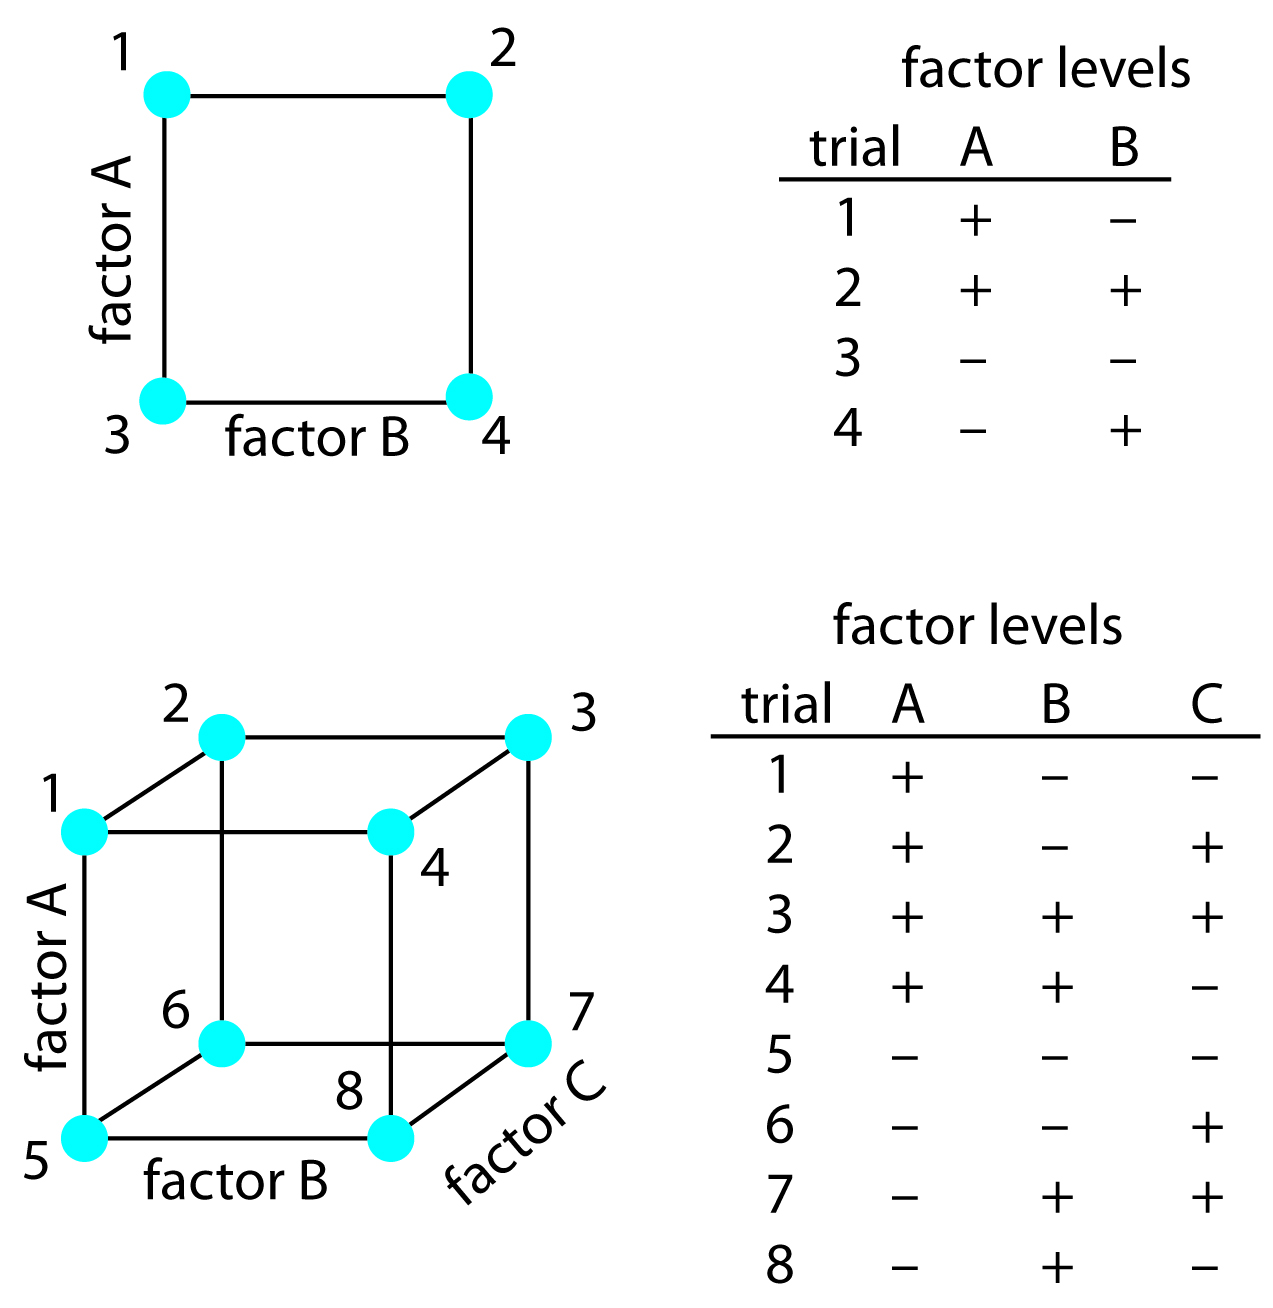
\includegraphics[width=0.7\linewidth, height=0.3\textheight]{art/full_factorial}
\caption[Full Factorial Design]{Full factorial designs: $2^2$ and $2^3$. \newline \url{http://chemwiki.ucdavis.edu/Analytical_Chemistry/Analytical_Chemistry_2.0/14_Developing_a_Standard_Method}}
\label{fig:full_factorial}
\end{figure}
With this $2^2$ design, we may recover several effects:
The effect of varying $A$ from $-$ to $+$: the \emph{main effect of $A$}.
The effect of varying $B$ from $-$ to $+$: the \emph{main effect of $B$}.
The effect of varying both $A$ and $B$ from $-$ to $+$. 

We typically denote $\mu_{(1)}$ the expected response for treatment $A=-,B=-$; 
$\mu_a$ for $A=+,B=-$;
$\mu_b$ for $A=-,B=+$;
$\mu_{ab}$ for $A=+,B=+$.
We can thus identify the following parameters:
the global mean $\mu$, the main effect of A $\tau^A$, the main effect of B $\tau^B$, and an interaction between A and B $\tau^{AB}$:
\begin{align}
	\tau^A &:= \frac{1}{2}\left( (\mu_{ab}+\mu_a)/2- (\mu_{(1)}+\mu_b)/2\right), \\
	\tau^B &:= \frac{1}{2}\left( -(\mu_{ab}+\mu_a)/2 +  (\mu_{(1)}+\mu_b)/2\right), \\
	\tau^{AB} &:= \frac{1}{4}\left( \mu_{ab} - \mu_a +  \mu_{(1)} - \mu_b \right).	
\end{align}



\marginnote{Interaction}

Slightly intruding into the realm of data analysis, a visualization of interactions is known as the \emph{interaction plot}, depicted in Figure~\ref{fig:interaction_plot}. 
The upper left panel demonstrates a lack of interaction (think why), while the upper right panel depicts an interaction.
\begin{figure}[ht]
\centering
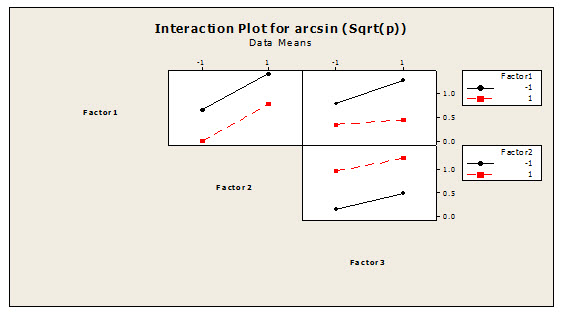
\includegraphics[width=0.3\textheight]{art/attribute_doe_interaction_plot}
\caption[Interactions plot]{Interactions plot. \newline \url{http://blog.minitab.com/blog/statistics-in-the-field/optimizing-attribute-responses-using-design-of-experiments-doe-part-2}}
\label{fig:interaction_plot}
\end{figure}


\begin{remark}[Screening Experiments]
The $2^k$ designs are probably the most popular full factorial designs. 
This may be attributed to the fact that many factors studied really have two levels, but more plausibly, since these are merely \emph{screening} experiments. 
Once non related factors have been screened, the experimenter may proceed from the $2^k$ design to more elaborate ones. 
\end{remark}



\begin{remark}[Intermediate Factor Levels]
In a $2^k$ design, a factor may actually be a continuous controllable input which was restricted to two values for convenience. 
After estimating the effect of the factor, we may want to know what would the effect have been, were we to set it on some intermediate level.
It is customary to assume that a main effect acts linearly in-between experimental conditions, yet you should remember that there is nothing in the data to support this.
For a more rigorous approach, see the Response Surface Methodology section (\ref{sec:response_surface}).
\end{remark}


\begin{remark}[Crossed Treatments]
Both crossover designs and full factorial designs are \emph{crossed} in that all factor combinations are sampled. 
The difference is that in a full-factorial, a factor combination is applied simultaneously to an experiment unit, and in a crossover design, the application is sequential \citep{everitt_cambridge_2010}.
\end{remark}



\subsubsection{$3^k$ Designs}
I think that the name $3^k$ design is rather self explanatory.
Then again, more than $2$ levels are rarely treated as factorial experiments. 
This is because $3$ level factors typically appear when aiming at optimizing the factor combination, for which the \emph{response surface} methodology of Section~\ref{sec:response_surface} is more economical.




\subsection{Fractional Factorial}
The full factorial designs are the simplest designs to setup and interpret. 
A major drawback, are the resources required when $k$ is large. 
This is where the \emph{fractional factorial}, or \emph{partial factorial} designs kick in.
The fundamental idea is to design a full factorial, but skip a couple experimental conditions. If conditions to skip are wisely selected, only information on higher order interactions will be compromised.


\begin{example}[From $2^2$ to $2^{(2-1)}$]
\label{eg:fractional_factorial}
As a first example, we will try to save some time and money by eliminating particular conditions of the $2^2$ design in Figure~\ref{fig:full_factorial}.
As the name may suggest, a $2^{2-1}$ design, has $2$ experimental conditions in each run. 
There are thus $\binom{4}{2}=6$ possible eliminations.
\begin{table}[ht]
\begin{tabular}{|p{2.5cm}|p{10cm}|}
\hline Elimination &  Problem \\ 
\hline
\hline 1,2 &  No information on $a$. \\ 
\hline 1,3 &  No information on $b$.\\ 
\hline 1,4 &  $a$ aliased with $b$ aliased with $ab$. \\ 
\hline 2,3 &  $a$ aliased with $b$ aliased with $ab$. \\ 
\hline 2,4 &  No information on $b$. \\ 
\hline 3,4 &  No information on $a$.\\ 
\hline 
\end{tabular} 
\label{tab:partial_factorial}
\caption[Aliasing]{Aliasing in a $2^{2-1}$ design: All possible eliminations from the $2^2$ design that lead to a $2^{2-1}$ design.}
\end{table}
\end{example}

The lesson from Example~\ref{eg:fractional_factorial} is that in a fractional factorial our savings in time and money, come at the cost of the information that can be drawn from the experiment.
The idea behind partial factorial experiments, is that by an informed choice of the conditions skipped, we can choose what information to give up. The information lost, is known as the \emph{alias structure}.\marginnote{Alias Structure}

In practice, we will rarely do the actual elimination of conditions, but rather revert to pre-selected designs. 
Table~\ref{tab:partial_factorial_ii}, generated with the \rcode{FrF2()} in the \rcode{FrF2} \R package, is an optimal $2^{3-1}$ design.
Using the \rcode{design.info()} function of that same package, we know that the aliasing structure of this design is
$a=bd=ce, b=ad, c=ae, d=ab, e=ac$.
We will not go into the details of how the aliasing structure is computed, but rather refer the reader to \cite{cox_theory_2000}.
\begin{table}[ht]
\centering
\begin{tabular}{rrrrrr}
  \hline
 & A & B & C & D & E \\ 
  \hline
1 & -1 & 1 & -1 & -1 & 1 \\ 
  2 & 1 & -1 & 1 & -1 & 1 \\ 
  3 & -1 & -1 & -1 & 1 & 1 \\ 
  4 & -1 & 1 & 1 & -1 & -1 \\ 
  5 & -1 & -1 & 1 & 1 & -1 \\ 
  6 & 1 & 1 & 1 & 1 & 1 \\ 
  7 & 1 & -1 & -1 & -1 & -1 \\ 
  8 & 1 & 1 & -1 & 1 & -1 \\ 
   \hline
\end{tabular}
\label{tab:partial_factorial_ii}
\caption[Fractional Factorial Design]{$2^{5-2}$ design.}
\end{table}


\begin{definition}[Resolution of a Design]
As we have already seen, there are $\binom{2^k}{2^{k-p}}$ possible eliminations that convert a $2^k$ design to a $2^{k-p}$ design.
We call the \emph{resolution of the design}, the lowest order effect that is aliased. 
In Table~\ref{tab:partial_factorial_ii}, the resolution is 1, making it a rather unattractive design. 
Resolutions below 3 typically considered not informative, and above 5, considered wasteful.
\end{definition}


\begin{extra}[Coding Theory]
There is a close relationship between design of experiments and coding theory in computer science. 
A possible reference on the matter is \cite{hill_first_1986}, or \cite{hedayat_orthogonal_1999}.
\end{extra}



\subsection{Split Plot Design}
\label{sec:split_plot}
A \emph{split plot}, or \emph{split unit} design, is essentially a factorial design with blocking. 
It takes its name from farming plots: where these are used for blocking and split among the various treatments. 
The canonical example is due to \cite[Sec.12.4]{montgomery_design_2012}, and consists of studying two production factors with blocking by day. 
For more on split plots see \cite[Sec.6.4]{cox_theory_2000}.



\section{Continuous Factors}
When dealing with continuous factors, or \emph{quantitative factors}, we have many more analysis strategies than when dealing with qualitative factors.
No matter the analysis strategy, it is still important of choosing the right factor level combinations to study.

Clearly, we cannot identify nonlinearities when sampling a factor only a two levels.
We may thus opt for a full $3^k$ factorial design to fit a non-linear surface to the data.
The factor encoding would typically be $\{-1,0,1\}$,
A full $3^k$ factorial design may however be needlessly expensive. 
A more common approach in industrial application is the \emph{central composite design}, where a $2^k$ design is augmented with well chosen sampling points. \marginnote{Central Composite Design}
For more details see \cite[Sec.6.6]{cox_theory_2000}


\subsection{Response Surface Methdology}
\label{sec:response_surface}
As the name suggests, \emph{response surface methdology} deals with the estimation of the response surface to the levels of continuous factors.
Response surfaces are typically assume to be (approximately) quadratic, and experimentation typically conducted in stages. First screening factors, then fitting a surface, and finding optimal factor levels.



\subsection{Taguchi Methods}
Taguchi methods is a collective name for the philosophy, design, and analysis methods in industrial applications promoted by Genichi Taguchi in 1970's Japan.
Focusing on the design principles, we may note the following particularities of Taguchi's method:
\begin{enumerate}
\item Achieving low variability is more challenging then achieving a target value. 
\item Factors which can be controlled in a lab, but not in production, are deliberately varied. Typically in split plot  designs (\ref{sec:split_plot}).
\item Systematic use of latin hypercubes to study main effects and two-way interactions. Particularly \emph{Plackett–Burman designs}.\marginnote{Plackett Burman Design}
\item Log variability is often used as the response.
\end{enumerate}





\subsection{Optimal Designs}
% 1D least squares example
% pD least squares example
% logistic regression example


Our discussion until now has been informal with respect to the desirable qualities of a design. 
We used the idea of ``balance'' and ``orthogonality'' to avoid bias and unwelcome variability.
In this section, we try to formalize the notion of a ``good design''.
We start with some motivating examples.

\begin{example}[Design for non linear regression]
\label{eg:design_linear}
Figure~\ref{fig:design_linear} demonstrates the effect of the different location of the sampling points ($x$) on the quality of the estimated regression line, in a \textbf{linear} model.
As the figure depicts, it is preferable to spread the sampling points as far as possible, as intuition may suggest.
\begin{figure}[ht]
\centering
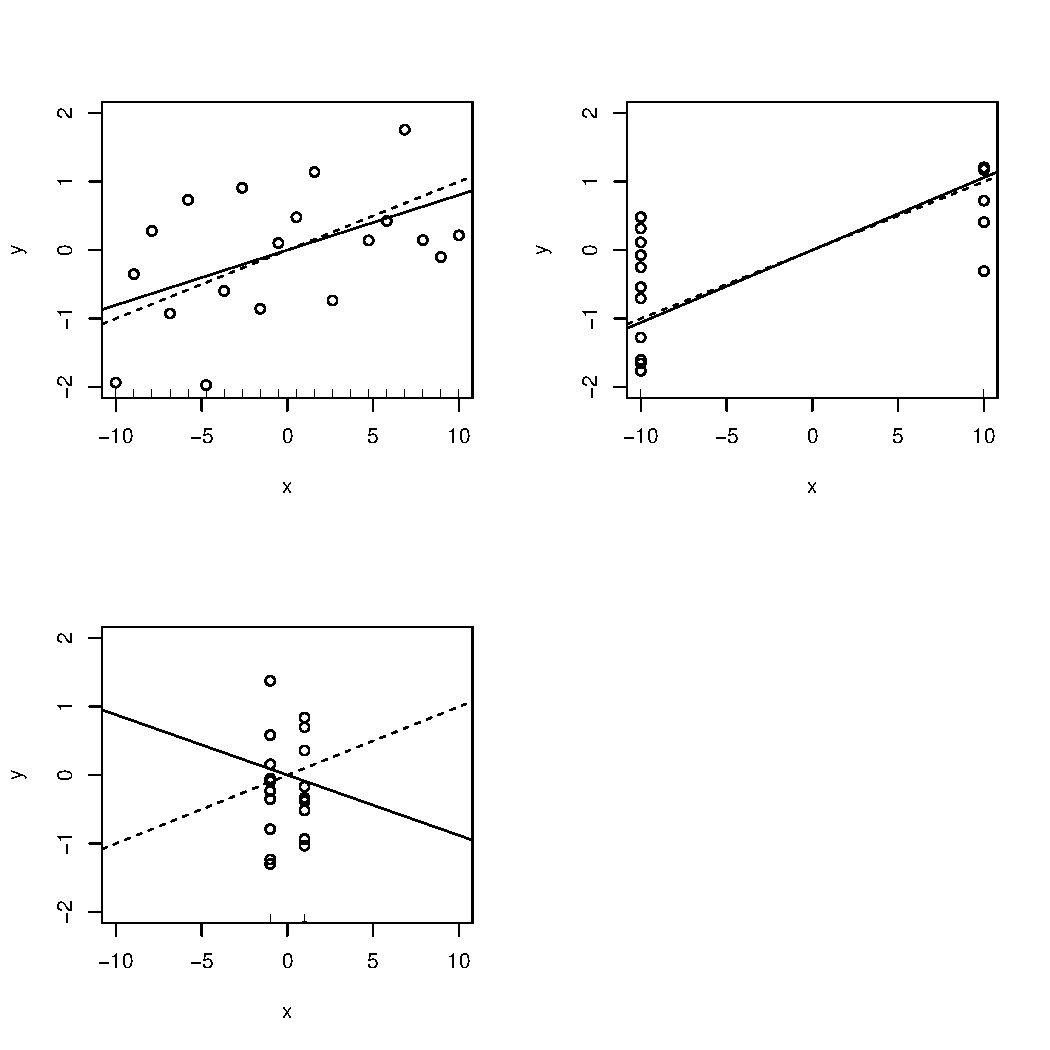
\includegraphics[height=0.3\textheight]{art/linear}
\caption[Design for Linear Models]{Design for linear regression. Different panels show different designs. True function as a dashed line. Estimated function as a full line.}
\label{fig:design_linear}
\end{figure}
\end{example}





\begin{example}[Design for non linear regression]
\label{eg:design_non_linear}
Figure~\ref{fig:design_nonlinear} demonstrates the effect of the different location of the sampling points ($x$) on the quality of the estimated regression line, in a \textbf{nonlinear} model.
The figure is non conclusive as to the best design, but it may seem that unlike the linear case (Example~\ref{eg:design_linear}) optimality is achieved in some non trivial sampling scheme.
\begin{figure}[ht]
\centering
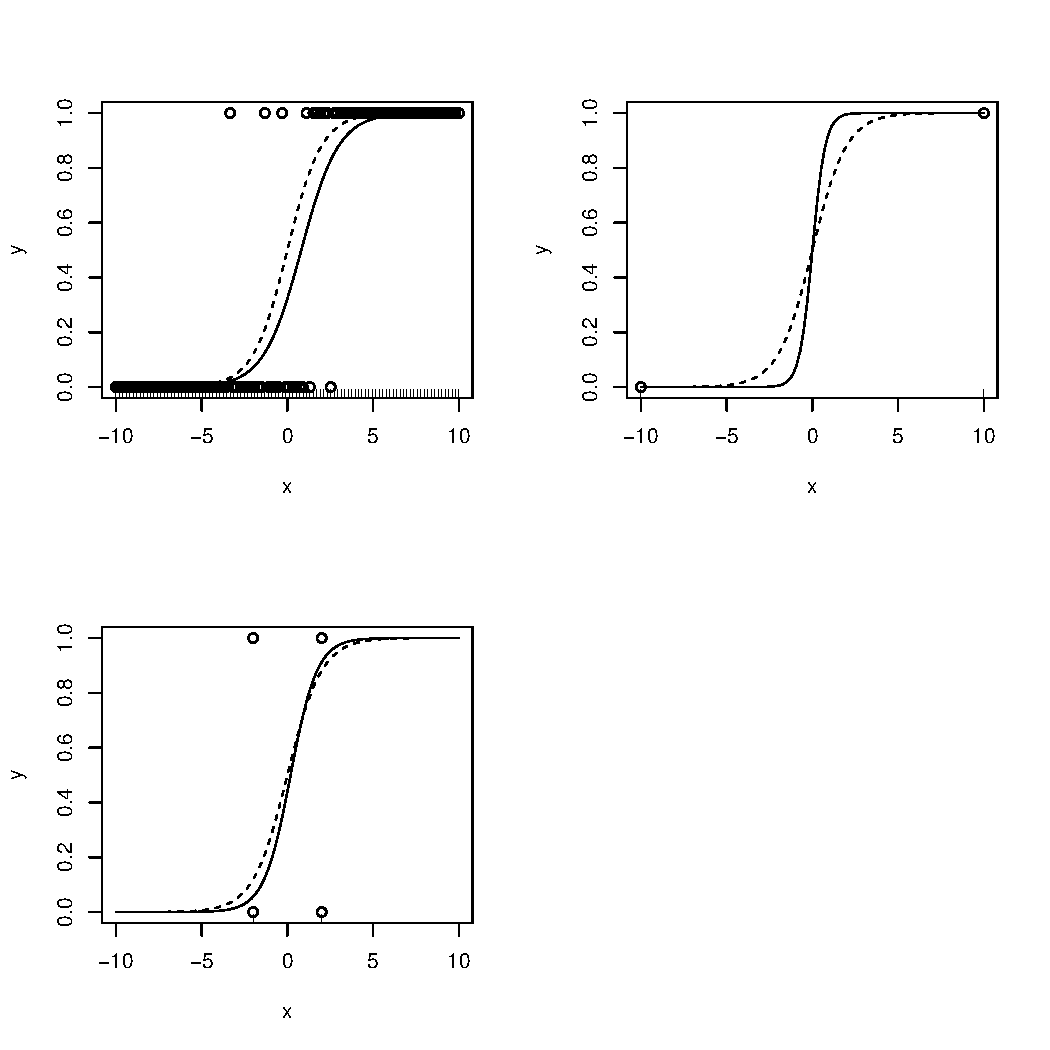
\includegraphics[height=0.3\textheight]{art/nonlinear}
\caption[Design for Non Linear Models]{Design for non linear regression. Different panels show different designs. True function as a dashed line. Estimated function as a full line.}
\label{fig:design_nonlinear}
\end{figure}
\end{example}





Now are some facts that are supported by the previous examples:
\begin{enumerate}
\item The idea of ``balancing'' as a design criterion is very useful with discrete factors, but limited with continuous factors. 
\item The optimal design may depend on the unknown generative model. Luckily, for linear models, this is not the case, and an optimal design will be so for all values of the generative parameter.
\end{enumerate}



\subsection{Space Filling Design}
\label{sec:space_filling}
The most natural of designs, which is particularly suitable when we have no a-priori assumption on the functional relation between the (continuous) factors, $f:x \mapsto y$,  and the response is known as a \emph{space filling design}.
As the name suggests, in a space filling design we aim at filling the factor space. Lacking any a-priori information, the filling will typically be as uniform as possible. 
We note however, that once information on $f$ is made available, then a space filling design is typically sub optimal (see Example~\ref{eg:design_linear}).

\begin{extra}[Space Filling and Hashing]
If you are familiar with the idea of \emph{hashing functions}, then you may see the similarity between space filling and the \emph{uniformity} property of hash functions. 
For a more rigorous discussion, see \cite{hill_first_1986}.
\end{extra}



\subsection{Covariance Optimality}
We have already noted the the optimality of the design depends on the data generating process.
In this section it is made obvious that optimality will also depend on the analysis method we choose.

When estimating the effect of a single continuous factor, we would like a design that gives us the most information per observation. This is the same as minimizing the variance of the estimator: $\min \{Var(\hat{\beta})\}$.

When generalizing to several continuous factors, with several effect, matters are more subtle.
This is because, having several parameters, we may consider several target criteria such as
minimal average variance, or minimal worst-case variance.
Matters further complicate when effect estimates are correlated, as will be promptly explained. 


\begin{definition}[Error Covariance Matrix]
For a $p$-vector of effects $\beta$, we define the $p \times p$ \emph{error covariance} matrix $M(\hat{\beta},\beta)$ to be 
\begin{align}
	M(\hat{\beta},\beta)_{i,j}:= \expect{(\hat{\beta}_i-\beta_i)((\hat{\beta}_j-\beta_j))}  
\end{align}
\end{definition}
Denoting $M=M(\hat{\beta},\beta)$, we readily note that for unbiased $\hat{\beta}$, then the diagonal of $M$ is simply the variances of $\hat{\beta}$, and the off-diagonal are the covariances. 
We also remark that if $p=1$, then $M$ is merely the scalar variance. 

We now try to generalize the idea of ``minimal variance'' to the multivariate case. 

\begin{definition}[A-Optimality]
	A design is said to be \emph{A optimal} if it minimizes the trace of $M$.
\end{definition}
A-optimality has an intuitive interpretation: since the average variance is proportional to the trace, then A-optimality is actually minimizing the average variance over effects.

Alas, A-optimality does not account for covariances. 
In an extreme scenario, if we have several copies of the same variable, the more copies we have, the more importance that variable will be given by A-optimality.
The most popular optimality criterion is known as \emph{D-optimality}, and does not suffer from this phenomenon.

\begin{definition}[D-Optimality]
	A design is said to be \emph{D optimal} if it minimizes the determinant of $M$.
\end{definition}
If you are familiar with the geometrical interpretation of the determinant, this definition may not surprise you. 
If not, then one way to think of D-optimality is via confidence regions.
D-optimality has the property that in the multivariate Gaussian case, a D-optimal design will return confidence regions for $\beta$ with smallest volume. 


\begin{extra}[Other Optimality Criteria]
There are as many optimality criteria as there are matrix norms. 
For a more detailed review, see \cite{wikipedia_optimal_2015}.
\end{extra}

The non-linear model example (\ref{eg:design_non_linear}) suggests that the optimal design may depend on the underlying (unknown) effect $\beta$. 
This is obviously bad news since if we had knowledge of $\beta$, we would not need an experiment to estimate it. 
There are, however, some good news.
First, for linear models and least-squares estimate, then $M$ will not depend\footnote{This is known as the \emph{equivariant in law} property.} on $\beta$, and neither will the optimal design. 
Second, when $M$ does depend on $\beta$, we will simply do some initial small experiment, and then optimize the design based on initial results. 



\section{Sequential Designs}
\label{sec:sequantial}
% Mark Vandelmeulenbruke

Consider a clinical trial with a treatment and control group.
Now assume the medicine being tested is a miracle cure with immediate improvement. 
Do we really need to keep administering placebos to the control group, just because that was the initial experimental design?
This is where sequential designs come in.
Interestingly, the initial application of a sequential design was not in drug testing, but rather in a military context \citep{wald_sequential_1945}.

The problem with sequential testing, is the \emph{type-I error inflation}, which is simply a \emph{multiplicity problem}. \marginnote{Multiplicity}
To see this, think about an endless sequential experiment. Also assume the null hypothesis is true. 
Can we agree that a regular (non sequential) experiment will not reject $H_0$? 
Can we also agree that a sequential experiment will necessarily reject $H_0$ at some stage?

In it simplest version, a sequential design allows early stopping for rejection of the null, or for futility (non-rejection). 
In more elaborate schemes then not only is early stopping allowed, but also the redesign of the experiment. 
This is known as \emph{adaptive design}. The crux, as usual, is not inflating the type-I error, or introducing bias, by redesigning.\marginnote{Adaptive Design}


\begin{extra}[Active Learning]
In the machine learning literature, the idea of adaptive design of experiments is known as \emph{active learning}, where the emphasis is less on adaptive-testing, but rather on adaptive-estimation.
\end{extra}




\section{Computer Experiments}
% no randomness
% space filling parameter choices for simulation
\begin{example}[Designing Wings]
\label{eg:wings}
Consider the problem of designing an air-craft's wing.
We would like to know how the wing's attributes, i.e., factors, govern its lift.
We could obviously conduct real-life experiments by varying the wing's attributes, building the wing, flying the air-plane, and recording results. 
Needless to say how expensive this process is.
It is much more reasonable to program the differential equations that govern the lift to a computer, fix several factors values, and solve the equations.
This is what \emph{computer experiments} are all about. 
\end{example}


The wind design example (\ref{eg:wings}) demonstrates the following points:
\begin{enumerate}
\item Computer experiments are essentially numerical solutions to complicated systems of equations.
\item Because solutions take a lot of time, only a small finite set of values may be evaluated. 
\item The ``response'' to each treatment, is deterministic. 
\item The problem of interest is in reconstructing the response at non measured factor values, so that optimal values may be identified. 
\end{enumerate}
It is thus not uncommon to call upon DOE theory for choosing the factor combinations to be experimented with. Space filling designs (Sec.~\ref{sec:space_filling}) being a particularly prevalent choice. 
The analysis of computer experiment is very different than real-life experiment since we have no noise component. 
See \cite{sacks_design_1989} or \cite{santner_design_2013} for further details. 



\section{Bibliographic Notes}
[TODO]